%!TeX root = pure_electroporation
\documentclass[fleqn,10pt]{paper}

\usepackage[left=2cm,right=2cm,
top=1.25cm,
bottom=1.5cm,%
headheight=11pt,%
letterpaper]{geometry}



\usepackage[left=2cm,right=2cm,
			top=1.25cm,
			bottom=2.25cm,%
			headheight=11pt,%
			letterpaper]{geometry}
			
\frenchspacing			

\nonstopmode




\usepackage{lmodern}
\usepackage[T1]{fontenc}
\usepackage[utf8]{inputenc}



\usepackage{noweb}

\usepackage{multicol}
\usepackage{fancyhdr}
\usepackage{blindtext,graphicx}
\usepackage[absolute]{textpos}
%\usepackage[parfill]{parskip}
\usepackage{parskip}
\setlength{\parskip}{\baselineskip}

\usepackage[colorlinks=true,citecolor=brown]{hyperref}
\usepackage{gensymb}
\usepackage{csquotes}
\usepackage{amsmath}
\usepackage{fontawesome}
\usepackage{orcidlink}
\usepackage{standalone}
\usepackage{pdfpages}
\usepackage{subfiles}
\usepackage{svg}
\usepackage{sidecap}
\usepackage{float}
\usepackage{amssymb}
\usepackage{textcomp}
\usepackage{lettrine}
%\usepackage[T1]{fontenc}

\usepackage{soul}


%\usepackage{draftwatermark}
%\SetWatermarkText{DRAFT}
%\SetWatermarkScale{0.25}

\usepackage{booktabs,caption}
\usepackage[flushleft]{threeparttable}

%\usepackage{biblatex}
\usepackage[backend=bibtex8, sorting=none, style=chem-angew]{biblatex}

\let\cite\footfullcite

%\let\cite\footcite

\addbibresource{processed.bib}
%biblatex has a zoterordfxml
% might avoid the need for python bibtex_collections.py



\usepackage{etoolbox}
\AtBeginEnvironment{quote}{\small}




\usepackage{pifont}
\newcommand{\cmark}{\ding{51}}%
\newcommand{\xmark}{\ding{55}}%


\newcommand{\citationneeded}[1][]{\textsuperscript{[\color{blue}{\it \bf{citation needed}#1}]}}
\newcommand{\dubiousdiscuss}[1][]{\textsuperscript{\color{blue} [{\it \bf{dubious-discuss}}]} }

\newcommand{\light}[1]{\textcolor{gray}{#1}}

%
%
\usepackage{titlesec}
%
%% custom section


\titleformat{\section}
{\normalfont\LARGE\bfseries}{\thesection}{1em}{}
%\titleformat{\section}
%{\normalfont\LARGE\bfseries\PRLsep}
%{{{{\itshape \thesection\hskip 9pt\textpipe\hskip 9pt}}}}{0pt}{}
%
%% custom section
%\titleformat{\subsection}
%{\normalfont\Large\bfseries\PRLsep}
%{{{{\itshape \thesection\hskip 9pt\textpipe\hskip 9pt}}}}{0pt}{}
%
%
%


\newcommand{\Wsqm}{$\text{ W/m}^2$}

\newcommand{\ghfile}[1]{\href{https://github.com/0xDBFB7/covidinator/tree/master/#1}{\faGithub/\url{#1} }}

%\newcommand{\supercite}[1]{}
%\newcommand{\supercollect}[1]{}


\newlength{\PRLlen}
\newcommand*\PRLsep[1]{{\itshape \Large\settowidth{\PRLlen}{#1}\advance\PRLlen by -\textwidth\divide\PRLlen by -2\noindent\makebox[\the\PRLlen]{\resizebox{\the\PRLlen}{1pt}{$\blacktriangleleft$}}\raisebox{-.5ex}{#1}\makebox[\the\PRLlen]{\resizebox{\the\PRLlen}{1pt}{$\blacktriangleright$}}\bigskip}}


\renewcommand{\thefootnote}{\textcolor{gray}{\arabic{footnote}}}


\usepackage{graphicx}
\graphicspath{ {../media/} 
				{../firmware/eppenwolf/runs/sic_susceptor/} 
			}

\usepackage{tcolorbox}
\newtcolorbox{protocol}{colback=yellow!5!white,colframe=yellow!75!black}
\newtcolorbox{equipment}{colback=orange!5!white,colframe=orange!75!black}
\newtcolorbox{autem}{colback=red!5!white,colframe=red!75!black}
\newtcolorbox{toolchain}{colback=blue!5!white,colframe=blue!40!black!40}
\newtcolorbox{sidenote}{colback=cyan!5!white,colframe=blue!40!black!40}
%https://tex.stackexchange.com/questions/66154/how-to-construct-a-coloured-box-with-rounded-corners

%\usepackage[sfdefault,light]{roboto}

\setlength{\TPHorizModule}{1cm}
\setlength{\TPVertModule}{1cm}





%%%%********************************************************************
% fancy quotes
\definecolor{quotemark}{gray}{0.7}
\makeatletter
\def\fquote{%
	\@ifnextchar[{\fquote@i}{\fquote@i[]}%]
}%
\def\fquote@i[#1]{%
	\def\tempa{#1}%
	\@ifnextchar[{\fquote@ii}{\fquote@ii[]}%]
}%
\def\fquote@ii[#1]{%
	\def\tempb{#1}%
	\@ifnextchar[{\fquote@iii}{\fquote@iii[]}%]
}%
\def\fquote@iii[#1]{%
	\def\tempc{#1}%
	\vspace{1em}%
	\noindent%
	\begin{list}{}{%
			\setlength{\leftmargin}{0.1\textwidth}%
			\setlength{\rightmargin}{0.1\textwidth}%
		}%
		\item[]%
		\begin{picture}(0,0)%
		\put(-15,-5){\makebox(0,0){\scalebox{3}{\textcolor{quotemark}{``}}}}%
		\end{picture}%
		\begingroup\itshape}%
	%%%%********************************************************************
	\def\endfquote{%
		\endgroup\par%
		\makebox[0pt][l]{%
			\hspace{0.8\textwidth}%
			\begin{picture}(0,0)(0,0)%
			\put(15,15){\makebox(0,0){%
					\scalebox{3}{\color{quotemark}''}}}%
			\end{picture}}%
		\ifx\tempa\empty%
		\else%
		\ifx\tempc\empty%
		\hfill\rule{100pt}{0.5pt}\\\mbox{}\hfill\tempa,\ \emph{\tempb}%
		\else%
		\hfill\rule{100pt}{0.5pt}\\\mbox{}\hfill\tempa,\ \emph{\tempb},\ \tempc%
		\fi\fi\par%
		\vspace{0.5em}%
	\end{list}%
}%
\makeatother







%%%%********************************************************************
%title link to doi
\newbibmacro{string+doiurlisbn}[1]{%
	\iffieldundef{doi}{%
		\iffieldundef{url}{%
			\iffieldundef{isbn}{%
				\iffieldundef{issn}{%
					#1%
				}{%
					\href{http://books.google.com/books?vid=ISSN\thefield{issn}}{#1}%
				}%
			}{%
				\href{http://books.google.com/books?vid=ISBN\thefield{isbn}}{#1}%
			}%
		}{%
			\href{\thefield{url}}{#1}%
		}%
	}{%
		\href{https://doi.org/\thefield{doi}}{#1}%
	}%
}

\DeclareFieldFormat{journaltitle}{\usebibmacro{string+doiurlisbn}{\mkbibemph{#1}}}

\usepackage{physics}
\usepackage{bm}
\usepackage{listings}
\newcommand{\bstar}[1]{ {#1}^{\bm*} }

 \pagestyle{empty}

\begin{document}




\title{Selective electroporation of the viral envelope via optimal control of transmembrane potential}
\author{\footnotesize{Daniel Correia\orcidlink{0000-0002-9353-0216} \{dcorreia@whimsysciences.com || therobotist@gmail.com\}
		 \href{https://0xdbfb7.com/email_pledge.txt}{Please don't hesitate to contact; see here}}\footnote{Ontario, Canada; contact information in the ORCiD.}}
\date{\small{March 21 2021}}

\flushbottom 
%%\maketitle
%\begingroup
%\let\center\flushleft
%\let\endcenter\endflushleft
\maketitle
%\endgroup



\thispagestyle{empty}

\renewcommand{\abstractname}{Summary}    % clear the title

\begin{abstract}
	\noindent The phenomenon of electroporation occurs when extreme applied electric fields in the MV/m range drive transmembrane potentials, leading to pores in (and potentially the destruction of) membranes. This is commonly harnessed for transfection into the cell in the laboratory, and has recently been shown clinically to be safe and effective for the in-situ ablation of tumors.
	
	\noindent As pulse duration is reduced from the microsecond to sub-nanosecond regime, effects targeting smaller intracellular structures are expected and observed, and a degree of tunability arises. Indeed, pulses shorter than 10 ns have been observed to porate the nuclear envelope and organelle membranes while leaving the plasma membrane intact.
	
	Fortuitous dielectric properties ostensibly due to the densely-packed genome core and apparently only affecting some ssRNA viruses 
	
	\noindent Recently-developed multi-gigawatt electrical pulse systems may offer a possible means of noninvasively propagating such pulses into deep tissues, such as within lungs. 
\end{abstract}

%send to jeff on the discord?

%mention the github again


\lettrine{A}{s} an addendum to a crude technical report \cite{notes2021} by the author, presenting some experimental results on an adjacent technique

In a continued effort to make ultracrepidarian physicists such as ourselves feel useful in the wake of a purely biological threat, and at the risk of producing more underpowered and scientifically useless results, 

\begin{tcolorbox}
While both mechanisms hinge on a set of time constants, those discussed in the previous paper referred to the time for viscous loss of energy into the surrounding medium and the normal modes of the viral envelope; here the time constants relate to capacitive charging, and Smoluchowski processes. Previously, the relevant quantities describing damage to the virion were mechanical displacement and membrane stress, whereas here we consider transmembrane voltage and pore diameter. 
\end{tcolorbox}

At the risk of self-plagarism, we will restate some precedent.

The idea of inactivating viruses via electric fields is not new. Very recently, Osorio \cite{Receptor2021} have reported on a susceptibility of SARS-CoV-2's spike protein to intense electric fields; however, in general, techniques targeting proteins appear to require truly extreme; fields of up to 2.9 GV/m were used in their computational study. Similarly, the dissocation of capsid proteins has been predicted by Man \cite{Picosecond2016b} at 2 GV/m.

These regimes of intensity may possibly be accessible via ultrashort optical techniques. Accordingly, Tsen \cite{Studies2014} report a non-electroporative mechanism, but these results have not been successfully independently replicated at that intensity\cite{No2011}. 

The field-induced breakdown of lipid membranes has proved to be a particularly useful property of the cell. From initial studies of crude membrane breakdown effects \cite{Reversible1979}

when a strong electric field is applied, they "...do enough things to justify international meetings, to fill a sizable book, and to lead one to speak of an entirely new technology for cell manipulation."

It is, in general, something of a singular outlier in that it is one of very few biological mechanisms that manifest at practical electric field intensities. Similar to thermal treatment, it also performs an operation something like integration with a threshold, a process distinct from normal absolute-value. It is perhaps this property which provides a small degree of tunability.

%\footnote{It is amusing to draw parallels between electroporation and Bialke et al's reports on spacecraft reaction wheels. In both cases, destructive process involve differential charging of the external shell (the spacecraft itself) against an internal shell (the reaction wheels), producing a potential difference across a highly resistive layer (a layer of grease on the ball bearings)}


Varactor-like parametric properties as the bilayer is compressed by forces from the potential difference. hydrodynamic

The same Debye screening effects are also of some relevance. 

Electroinsertion of proteins into membranes\cite{Clinical1996}; to provoke a local immune response near diseased tissues, 

The same electrostatic effects on lipid bilayers have been investigated for decades. Many extremely fascinating hydrodynamic and parametric 



Electroporation\cite{Electroporation1988}, now a common laboratory procedure, occurs when an enormous electric field causes ions in solution to diffuse across a cell membrane, capacitively charging it, provoking a change in lipid bilayer conformation\cite{Membrane2016}, either reversibly rendering the membrane permeable or, if the number and size of pores is considerable, the membrane may be permanently destroyed. This is one among many other, more subtle mechanisms; the minutia of poration can become extraordinarily complex in certain circumstances and are beyond the author's current understanding\cite{Theoretical2007}. Hydrodynamic

Therapies based on irreversible electroporation\cite{Nonthermal2013}\cite{Lipid2017} have recently been used in the clinic\cite{Irreversible2013} for tumor ablation. There is much discussion on electroporation as an alternative to viral vectors, but we have found surprisingly little discussion on clinical treatment of viral infection with these conventional electroporation therapies.

As in the previous paper, we must stress that meaningful bioelectrics research hinges very strongly on experimental design and methodology, and very few results can be trusted implicitly. It appears to be very difficult to unambiguously determine effects and their cause on a system as complex as a cell, especially when electrodes are in contact with solution and release an energy-dependent dose of metal ions.

However, long pulses at $\approx10$ MV/m appear to electroporate large enveloped viruses, similarly to host cells\cite{AC2017}

%There is a single report of the electroporation of HIV in the gray literature. This one of very few reports involving the electroporation of viruses, reporting the ~95\% inactivation of HIV using a standard commercial Bio-Rad electroporation system at 2.3 MV/m. However, the authors appear to have committed such an egregious breach of research ethics that we cannot cite them here.

 which we believe might hint that a regime of intensity, duration, and pulse count may exist to target the viral envelope. 
 
Despite considering the presumably harder problem of electroporating small lipid vesicles while inside the cell, rather than in extracellular fluid, \cite{Electroporation2013} report that 250 nm liposomes should be porated without inducing damage to the host cell, and their modelling shows that 100 nm liposomes may be porated by 4 ns pulses never exceeding 20 MV/m. 

The same field intensities do not appear to damage phages with protein capsids\cite{Manipulation2013}, in line with our previously-reported negative results on T4.

Capsid and envelope permeablization with 120 pulses, 500 ns each, at 3 MV/m, has been previously observed\cite{Inactivation1990}, but the RNA damage suggests that this is an electrochemical artifact \cite{Formation1996} (c.f. \cite{Microwave1987}). 

The trapping experiments we use were conducted at 


As in the previous paper, bulk dielectric properties of tissues are given by Gabriel. 


Pulse count and inter-pulse timing is another free variable. Joshi et al \cite{Selfconsistent2001} model that a carefully timed second pulse can have greater effects than a single pulse, in agreement with experiment on E. coli.

This seems to hint that electroporation occurs at the same order of magnitude field as host cells.

Of course, unlike localized tumors, viral infections are systemic, affecting many of the most favoured organs. 

Also be of some use for testing and detection. 



Note that, despite excellent evidence in [nanosecond review], microsecond in vivo and clinical treatment, nanosecond in vivo conduction, and, The NATO review concluded that evidence did not support non-contact, "electrodeless", even above the thresholds that might otherwise be expected to cause electroporation. has not yet found any evidence demonstrating electroporation via pulsed RF. 

de Seze, 

that said, the reviews of the ICNIRP [that 18 GHz  paper]

This property is 
\cite{Nanosecond2006b} 


This seems too simple.

Viruses have extraordinary mechanical properties (why is this? What selection pressures drive the selection of this pressure?), so it seems reasonable to speculate that their dielectric properties could differ substantially from those of other biological structures. 

In the extreme case of coliform bacteriophage, the genome is packaged so tightly into the protein capsid that the core is most accurately described as a glassy crystal of DNA\cite{Conformation2007}. ssRNA viruses like coronaviridae might be expected to be somewhat more sedate in packing density, but this does not seem to be borne out in the core conductivity data.

On the other hand, the eukaryotic "structome" also contains countless vesicles and structures of similar nature that might plausibly be damaged; small pockets of lipid in the endoplasmic reticula - nuclear pore complexes, etc. This appears to be seen to some degree in Gabriel's data; dense tissues exhibit a high cole-cole alpha coefficient [double check this]. It may not be possible to meaningfully predict all possible off-target effects, much like in drug discovery.


\section*{Basic scaling laws}

The most obvious difference is scale. All other properties of the system being equal, the standard Schwan equation for transmembrane voltage, $\Delta \phi = (3/2) E R \cos(\theta)$ implies that the steady-state DC voltage is proportional to the size of the particle. In the case of a 100 nm virus, this would 400x difference, which is reflected precisely in the steady state numerical simulations that follow.

Madiyar's Vaccinia electroporation data aligns with. Assuming that the host becomes permeable at 0.05 MV/m, the 250 nm vaccinia might be expected to have a threshold of 4 MV/m. Mutatoyo's data also agree roughly.  

This does not agree with Yamada \cite{Electroporation2012}'s data on electroporation of Hepatitis B.

A normalized (note that the true value of the virus' transmembrane voltage is, again, a factor of 400 reduced).

\begin{figure}[H]
	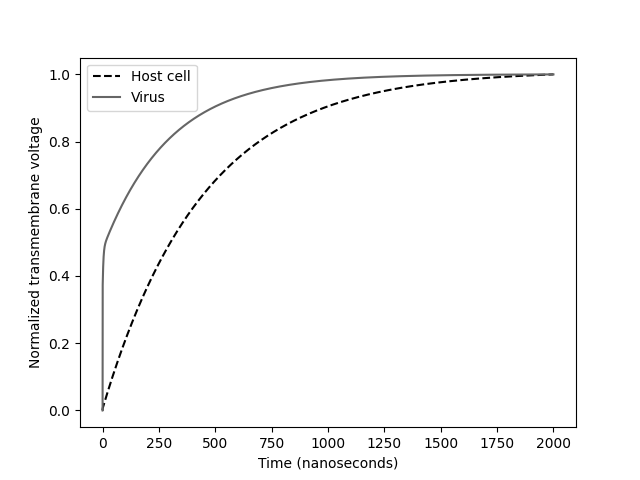
\includegraphics[width=\textwidth]{step_course}
\end{figure}


Despite the two having similar time constants (host: $\tau_1=444\ \text{ns},\ \tau_2=2.3\ \text{ns}$, virus: $\tau_1=295\ \text{ns},\ \tau_2=3.1\ \text{ns}$), the time course of the transmembrane voltage is clearly distinct. (Plot generated via the convolution method, \ghfile{transmembrane_steady_state.py})


Consider the following bipolar gaussian waveform, each with a FWHM of 500 picoseconds, separated by 1 nanosecond. In this case, the peak virus transmembrane voltage is no longer 1/400 less than the host cell, but 1/6.5, and the total energy in each curve is also improved to a ratio of 1/37. The second, inverted pulse has the effect of quickly zeroing out the host cell's decaying potential to improve the virus' energy ratio.

\begin{figure}[H]
	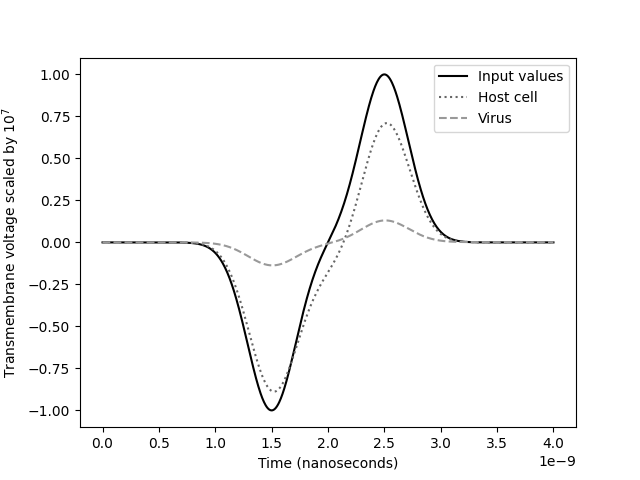
\includegraphics[width=\textwidth]{gaussian_pulse}
\end{figure}



%1/(250e-9 / 20e-6)



However, not field-time product [analytic, ]. 


[gaussian pulse results, 1/2.7]. 


There are two characteristic time constants; a low and a high-frequency one.

Some extremely simplified scaling laws for membrane charging effects due to short (sub-first time constant) pulses are given by Schoenbach \cite{Bioelectric2007}. This is based primarily on an equivalent circuit model, we largely neglect the electrodynamics that apply with short pulses and also the conductivity change due to pore formation, modelled by [insert equation from "ADC" paper]. Electroporation is a highly nonlinear effect\cite{Letter1974}, and this .

The membrane charging time constant from a single-shell model \cite{Ultrashort2004} - simplified for the low-density case. As the fraction, and papers citing this usually mention that this may not be representative of charging time in tissue.

$$\tau_c = \left(1 \frac{\rho_{medium}}{2} + \rho_{internal}\right) C_m (D/2)$$

where $\rho_{medium}$ and $\rho_{internal}$ are the resistivities of the medium and internal fluid (the cytoplasm for cells, and assumed to be the 'core' for viruses). Note that this time constant is unrelated to the relaxation time constant discussed in the previous paper, which was purely mechanical. \cite{Bioelectric2007} eq. 15, 

$$\Delta V_M = \frac{3}{2}\frac{E\tau D}{2 \tau_c }$$

substituting,

$$\Delta V_M = \frac{3}{2}\frac{E \tau}{C_m ((\rho_1/2) + \rho_2)}$$

that is, all else being equal, the induced transmembrane voltage appears to be invariant with particle diameter - mildly contrary to Rjif's more detailed analysis.

The viral envelope capacitance per unit area, $C_m$, can be determined simply by parallel-plate (Ermolina \cite{Study2001}); $C_m = (k\epsilon_0) / d$, where d is the membrane thickness. The cell and nucleus membrane have similar capacitance, but greatly differ in conductivity. 

Regrettably, despite their diminutive radii, viruses and host cells may well have overlapping time constants due to the other dielectric properties. However, even in the case where both time constants are nearly equivalent, a marked discrepancy in the time evolution of short pulses can be seen.

There may be an existing transmembrane potential that must be added - this is neglected in this case.


\section*{Empirical dielectric properties}


The dielectric properties of viruses have been determined by the fascinating and ingenious techniques involving electrorotation, dielectrophoresis, and dielectric spectroscopy. To prevent fluid heating, these are often conducted in low osmotic strength media; as enveloped viruses are permeable to small ions, some results may not necessarily representative of conductivities in physiological conditions or must be \cite{Assessment}.

The internal core permittivity of viruses is often referred to as being about 5 to 3 (Brackley \cite{Electrostatic2020}, SARS-CoV-2; and Schnelle \cite{Trapping1996}, Sendai and Influenza A) - however, Gimsa \cite{New1999}, on influenza report that the internal $\epsilon_r$ is probably closer to 30. Hughes on HSV-1 originally suggest 80\cite{Manipulation1998}, then refine to 30\cite{Dielectrophoretic2001}. We have not investigated this discrepancy. The internal osmotic strength of some viruses depends direclt on the growth medium's osmotic strength\cite{Osmotic2003}, so results with different media may not be comparable. Aggregation of viruses may also be a relevant artifact. 

Via electrorotation, it is usually found that the viral shell has a permittivity of about 60 to 80, similar to the nuclear envelope (60 to 100) but massively unlike the cell membrane ($\epsilon_r\approx 10$). This is very remarkable, since the lipid bilayer itself is somewhat similar in composition to the host cell, and the proteins that are stuck into it permittivity is generally assumed to be only about 4. Envelope, spike and membrane proteins may perhaps account for the discrepancy?!?

On the other hand, \cite{Electrostatic2020a} use a membrane value of 4.

Equivalent circuit models want to more accurately represent the - most importantly, the core permittivity intuitively seems like it should alter the reflection significantly at high frequencies, but isn't usually treated 

Influenza has a membrane thickness of about 4 nm (Harris \cite{Influenza2006}). However, Gimsa and Hughes use a shell thickness of 18 and 15 nm, respectively, to account for the membrane proteins and hemaglutinase. The $C_{envelope}$ may therefore be expected to fall within the range $2.9 \text{ to } 17.7 \text{ uF/cm}^2$.

Dry-weight measurements seem to suggest that influenza contains about 60\% water by weight \cite{lauffer1944biophysical}. Has diffusion coefficients and maintains a Donnan ion size equilibrium similar to that of lipid bilayers \cite{Effect2015b}. 

% should this be noweb python? python isn't really unit aware though
% maybe sympy or something?
% ooh we could have the supplemental appendix written right inline with noweb, 
% also python could print the equation back to latex

% Viral envelope capacitance per area:
% >>> (80 * electricConstant) / 4 nanometers -> 17.7 uF/cm^2
% >>> (60 * electricConstant) / 18 nanometers -> 2.9514 uF/cm^2
% Actual envelope capacitance:
% >>> 17.7 uF/cm^2 * 4 * pi * (50 nm)^2 -> 5.56 fF
% >>> 2.95 uF/cm^2 * 4 * pi * (50 nm)^2 -> 0.92 fF
% Actual envelope resistance:
% 



Critically, Gimsa and Schnelle data, both on influenza, seems to suggest a core conductivity of 0.8 to 0.1 milliSiemens/m (1000 to 10000 $\Omega \cdot m$), using a medium conductivity of 74 mS/m and 3 mS/m, respectively. This is far less conductive than cytoplasm or nucleoplasm, each on the order of 1 S/m (1 $\Omega \cdot m$) \cite{Study2001}. 

% if this is correct, scaling linearly:
% like 60 % water in core  * (1 S/m / 0.074) would get us to 1 mS/m.

% absolute pessimistic, using 0.8 mS/m and Schnelle's medium conductivity, would get us 0.008 * 0.6 * (1/0.003) = 1.6 S/m

However, Hughes suggests 30 mS/m for HSV-1, a significant discrepancy. Unlike influenza, HSV-1 has a complete protein capsid rather than a helical nucleocapsid. Protein capsids are typically regarded as monolithic and impermeable, whereas enveloped viruses are permeable, and therefore the ionic strength of the medium may be very important. No other sources of data on permittivity ion mobility in enveloped viruses were found.  \footnote{Special thanks to Professor Jan Gimsa for replying to my email!}

The viral envelope appears to be slightly less conductive than the cell membrane (0.1 $\micro$S/m \cite{New1999} vs 10 $\micro$S/m \cite{Study2001}), and far less conductive than the nuclear envelope (0.1 $\text{m}$S/m \cite{Study2001}).
%This ratio is the relevant quantity to find the steady state transmembrane voltage for long pulses (before pore conduction becomes relevant). gotta look into "interfacial / surfaec conductance"

% is the relaxation time quoted in some papers the one we're looking for here? alfalfa is 600 ns, is that a better, more direct value?

The dielectric properties of viruses do appear to differ considerably from the host, the discrepancy mainly in the internal core conductivity and perhaps the envelope permittivity. Despite this, because of the small radius of the virus, the first time constant of the virus transmembrane might plausibly range anywhere between 50 ns and 90 us, compared to between 100 ns and  for the both the plasma membrane and the nucleus.

% Virus time constant:
% >>> (((1 ohm m) / 2) + (1000 ohm meter)) * 2.9 uF/cm^2 * 50 nanometer -> 1.45 us
% >>> (((1 ohm m) / 2) + (10000 ohm meter)) * 17.7 uF/cm^2 * 50 nanometer -> 44.25 ns
% Host time constant:
% (already given by others, 100 ns)
% Nucleus time constant:
% using data from feldman paper,
% (Must be very careful regarding S/m, mS/m, etc!)
% >>> (((1 ohm m) / 2) + (1 ohm meter)) * 1.5 uF/cm^2 * 3 um -> 67.5 ns
% that's interesting, because it conflicts somewhat with shoenbach's suggestion that the nucleus has a longer time constant.

%At first glance, this may seem unfortunate: the host will be electroporated far before the virus.
%However, if a monopolar pulse train with a pulse duration shorter than the cell time constant, an intensity too low for, and a repetition rate of some 3 us, (200 khz), 



%%%%%%%%%%%%%%%%%%%%%%%%%%%%%%%%%%%%%%%%%%%%%%%%55
\subsection*{Error in Kotnik}

\begin{tcolorbox}
	
	There appears to be a minor typographical error in equation 8, transfer function, from Kotnik \cite{Time1998}. The equation is given in terms of a and b coefficients,
	
	\textcolor{red}{$$F(s) = \frac{a_1 s^2 + a_2 s + a_3}{b_1 s^2 + b_2 s + b_3} \text{ (eq. 8)}$$}
	
	whereas the correct order appears to be:
	
	\textcolor{blue}{$$F(s) = \frac{a_3 s^2 + a_2 s + a_1}{b_3 s^2 + b_2 s + b_1}$$}
	
	The rest of the paper appears to obey this coefficient order: for instance, equation A6e in that paper, in the derivation of the step function:
	
	$$E(s) = \frac{1}{s}$$
	
	$$F(s) \cdot E(s) = \frac{a_3 s^2 + a_2 s + a_1}{b_3 s^2 + b_2 s + b_1} \frac{1}{s} = \frac{a_3 s^2 + a_2 s + a_1}{b_3 s^3 + b_2 s^2 + b_1 s} \text{ (eq. A6c)}$$ 	%confirmed with mathematica.
	
	We will continue to use this convention, assuming the subscripts on equations 9a through f are correct. 
	
	This minor transposition was only detected late in the project, so some documentation in the repository may still contain the incorrect coefficients. Beware.

\end{tcolorbox}
%%%%%%%%%%%%%%%%%%%%%%%%%%%%%%%%%%%%%%%%%%%%%%%%55



\subsection*{Electrodynamic considerations}

Kotnik note an important fact: all these permittivity and conductivity values will also depend on frequency, which is not included in their model. We have not examined whether these factors can be extracted from existing plots. Also disregarded are the Poisson-Boltzmann shielding space-charges that proved all-important in the last study. 

The necessity for the Laplace transform over the Fourier-based method used for the precursor propagation in the previous report is founded in the requirement for a fully transient solution with a definite t=0.

The concept of optimizing an electroporation pulse is not novel, having been discussed by many groups in the past; either to produce different sterilization effects, tee Retelj use a series of, to 

\subsection{Attempts to solve for the optimal pulse in the s-space; convolution integral}

We must apologize once again to the mathematicians for sins of terminology and rigor.

This bears considerable similarity to e.g. radar waveform design and compressed sensing; problems of coherent control of quantum systems, single input multiple output underactuated robotics, simultaneous stabilization\cite{results1984}\cite{Simultaneous2005}.

a double integrator 

In many cases, the optimal (minimum-energy) control is equal to the transfer function

Scipy has a convenient LTI class that accepts the terms.



There are suprisingly many more quan

two plant

The time-domain response can be obtained from the step or impulse response function by evaluating the convolution integral, or by manually integrating the differential equation via some integrator.

In the previous paper, an analytic method was shown using variational calculus / lagrange multiplier. Unfortunately, while closed-form solutions appear to be readily available for some simplified cases (such as when the membrane is infinitesimally thin or when permittivity is neglected) [schwan paper], 

Kotnik discuss the transmembrane voltage due to several pulse shapes constructed simply from the Laplace Transform of the original differential equation. 

There appears to be an error in; the coefficients are in descending order, whereas they should be in ascending order. See 

Talele offer their own response due to an arbitrary waveform using the step response and a convolution integral \cite{Nonlinear2007}.

The impulse response is the derivative of the step response. The convolution integral (or sum, in the discrete case) can be performed either with the derivative of the input function and the step response, or the impulse response and the input function as algebraic convenience demands. Unfortunately

There exists an alternative convolution technique, due to the Convolution Property of the fourier transform.

Via Mathematica, the Fourier transform of both the impulse response and the step response exist, are analytic and of manageable size; however, the integral of the cost function is extremely unwieldy.


Pole placement

\subsection*{Nonlinear model predictive control, quadratic regulators, }

\subsection*{Frequency-domain solution}

Subtracting the frequency domain of the step responses of the two produced an interesting pulse, but not nearly optimal.

%polarization? can we somehow twist the polarization?

\subsection*{Pseudospectral solvers}

% is this direct or indirect method?

%An excellent overview of solutions http://plato.asu.edu/sub/nlounres.html - nah, not really that good

For use with GEKKO, the transfer function was converted into a system of differential equations:

For PSOPT, a further modification was needed, as the library does not appear to natively support the second derivative of the control; the second derivative was used as the control, and input into a differential-algebraic equation form.

Because the problem depends on the second derivative of sub-nanosecond curves, base variable and coefficient scaling varies by more than 20 orders of magnitude. 

PSOPT [] with IPOPT\cite{implementation2006} solver. PSOPT has the advantage of semi-automatic scaling based on supplied bounds. 

Both PSOPT and GEKKO's APMonitor backend use the famous ipopt solver. A number of linear solvers can be used. LANL's Tasseff's integration with the SPRAL solver, reportedly faster on large problems, was . HSL libraries ma57 and ma97 were used.

It was found very useful to test the equation setup by first propagating a test using a standard integrator (PSOPT's rk4 or mode 4).

A hard-to-detect lack of convergence would often produce a fallacious simulated output from PSOPT. To double-check that the solution was actually valid, the output was fed through the convolution integral method.

Considerable difficulty was encountered. 

An objective function with a constant integral control power constraint, $t_{end} = \int_0^{t_{end}} u(t)^2 dt$ was used, but this did not appear to yield meaningful results.

\subsection*{Optimal control solvers}



% need to check the required tolerances on the output - how stable is the solution


iLQR. Differential dynamic programming was not evaluated (julia lib).




\subsection*{Nondimensionalization}

The coefficients all have a very small value in standard units. Numerical error was presumed to account for at least some of the difficulty in optimization, so was partially nondimensionalized. 

the a and b coefficients both have units     

\[ \{\text{meter}\cdot \text{siemens}^2, \  \text{farad}\cdot \text{meter}\cdot \text{siemens} ,\ \text{farad}^2 \cdot \text{meter}\} \]

in physical units, typical values for as an example, \\
\verb|Cell(0.3, 80, 0.005, 30, 1e-8, 60, 50e-9, 14e-9, t)| \

$$R = 2.5\times10^{-8}$$
$$a_1 = 6\times10^{-26}$$
$$a_2 = 9\times10^{-33}$$
$$a_3 = 2\times10^{-41}$$
$$b_1 = 4\times10^{-26}$$
$$b_2 = 1\times10^{-32}$$
$$b_3 = 4\times10^{-41}$$

An input control waveform u(t) (volts per meter), and two output waveforms, $x_V(t)$ and $x_H(t)$ in volts.\\

%virus.__dict__

First system of differential equations (named V):\\

$$\dv[2]{x_V}{t} = 
\frac{R_V a_{1V}}{b_{1V}} \dv[2]{u}{t} 
+ \frac{R_V a_{2V}}{b_{1V}}  \dv{u}{t} 
+ \frac{R_V a_{3V}}{b_{1V}}  u
- \frac{b_{2V}}{b_{1V}} \dv{x_V}{t}
- \frac{b_{3V}}{b_{1V}} x_V $$


In practice, the solver takes a DAE: the second differential equation is split into an explicit system of eqs:

$$u1 = \dv{}{t} u$$
$$u2 = \dv{}{t} u1$$


$$x1_V = \dv{}{t} x0_V$$
$$x2_V = \dv{}{t} x1_V$$


Another system is solved simultaneously (named H), of identical form but different coefficients:

$$\dv[2]{x_H}{t} = 
\frac{R_H a_{1H}}{b_{1H}} \dv[2]{u}{t} 
+ \frac{R_H a_{2H}}{b_{1H}}  \dv{u}{t} 
+ \frac{R_H a_{3H}}{b_{1H}}  u
- \frac{b_{2H}}{b_{1H}} \dv{x_H}{t}
- \frac{b_{3H}}{b_{1H}} x_H $$


%x2  = (R*a1*u2 + R*a2*u1 + R*a3*u0 - b2*x1 - b3*x0)/b1

\subsection*{Nondimensionalization}

Let $x_V^{\bm*} = \frac{x_V}{x_{VK}}$ and $t^{\bm*} = \frac{t}{t_{K}}$ where $_K$ denotes a nondimensionalization constant (standard convention of $t_0$ is changed to $t_K$ to avoid confusion with subscript 0s used in simulation). (the forcing functional u is dependent on t, but this is implied).\\ \\

$$\frac{d^n}{dt^n} = \frac{1}{{t_K}^n}\frac{d^n}{d{\bstar{t}}^n}$$\\


$$ x_v(t) = A_v \frac{d^2u(t)}{dt^2} + B_v \frac{du(t)}{dt} + C_v u(t) - D_v \frac{dx_v(t)}{dt} - \frac{d^2 x_v(t)}{dt^2} $$ 

$$ x_h(t) = A_h \frac{d^2u(t)}{dt^2} + B_h \frac{du(t)}{dt} + C_h u(t) - D_h \frac{dx_h(t)}{dt} - \frac{d^2 x_h(t)}{dt^2} $$ 


% https://math.stackexchange.com/questions/3435173/how-to-nondimensionalize-a-second-order-differential-equation
% http://math.colgate.edu/~wweckesser/math312Spring05/handouts/Nondim.pdf
% https://faculty.math.illinois.edu/~rdeville/teaching/558/nondimensionalization.pdf
% http://math.colgate.edu/~wweckesser/math312Spring05/handouts/MoreNondim.pdf


% Kronbichler et al suggest an interesting method of nondimensionalizing.

% https://www.math.colostate.edu/~bangerth/publications/2008-boussinesq.pdf


GEKKO's .dt() operator allows u0 to be chosen as the control. 
Otherwise, the DAE form requires u2 to be used as the control.

A system of first-order Differential-Algebraic Equations:

Smooth noise-free combined filter and differentiator.

mayer (endpoint) or Lagrange (integral)

An advantage of bang-bang or bang-singular-bang over is that the values of u0 are not free. In PSOPT and , it was often found that (perhaps due to poorly-chosen values of the penalty factor rho, a poor initial guess, or some other issue in the problem setup), the gradient descent would decrease the control magnitude to a value below numerical accuracy. This necessitated a Lagrange constraint on the integral, further increasing the computational complexity and restricting the class of solutions. 



\subsection*{Analytic solution}


However, this overlooks a much simpler method.

Setting say, the logistic equation, produces an overdetermined system. using the above as a constraint in PSOPT was also ineffective.

\begin{tcolorbox}
	First instinct might be to try to solve for the waveform that sets alpha beta gamma to zero; feeding this though produces a reasonable solution []. 
\end{tcolorbox}

\subsection*{Hampath bang-bang control}

A good review of advanced bang-bang control techniques \cite{Computations2004}. 

Puts much more effort into further analytical rearrangement before resorting to; by more fully using Pontryagin's Maximum Principle, and by formulating a control theoretic Hamiltonian. What looks to be a superb code hampath, did not have the experience to implement the hamiltonian at short notice.



\subsection*{Niemann's bang-bang control control}

Niemann describes a straightforward bang-bang formulation using gradient methods, using gradient projection to implement the required boundaries \cite{Determinationa}. Because the unit step function of the transmembrane voltage is analytic, a bang-bang control can be simulated without integration, by simply summing the (as described by Kotnik). This appears to automatically resolve "backwards-integration" and sorting issues presented in chapter 3 of Niemann's thesis.

While 




\section*{Sensitivity analysis}

\section*{Limitations and recommendations for further study}



Extremely speculative and 

As previously mentioned, electroporation is rarely seen in non-contact studies. It is possible that some nuanced 

Involves careful control of the second derivative of a waveform 

Viruses vary by \%x . optimal over a distribution of cells and viruses. 

"Bulk effects", as the concentration increases, can completely alter the. It may not be possible to produce a robust enough scheme 

sensitivity analysis


must necessarily operate "open loop", without feedback, towards the transmembrane voltage



\subsection*{Software used and evaluated:}

casADi;

typeset in LaTeX on TeXstudio and Gummi.





\subsection*{Recommended reading}

de Seze; 

The book Scaling of Differential Equations is an excellent guide to the numerical treatment of DEs.

\section*{Commentary and discussion}

In easily mutable versions of this paper, this section will be 



I have been lucky to have been provided the opportunity to conduct this research. 



\end{document}